% Şablon otomatik olarak kapak ve onay sayfalarını sizin esogu.cls dosyasında girdiğiniz bilgilere göre oluşturmaktadır. Lütfen o dosyadaki "TEZLE İLGİLİ Bilgileri burada giriniz." bölümünü doldurunuz. 

% Eğer Tezinizi bu dosyada yazacaksanız "TEZİNİZİ BURADAN SONRA EKLEYİNİZ" bölümünden sonra ekeleyebilirsiniz. Özet ve Summary bölümleri /bolum klasörünün içindedir. 





\documentclass[]{esogu}			%Optionlar boş olacak, şablonu kullanmak için
\usepackage{lipsum}				%Anlamsız metin yazmak için
\bibliography{Zotero.bib}

%----------------------------------------------------------------------------------------
\begin{document}
\frontmatter %roma rakamları ile yazdırmak için
\title{OGU deneme}
%-----Dış kapak Türkçe---------- Burayı değiştirmeyin
\begin{titlingpage*}
\begin{center}
\footnotesize


	\begin{vplace}							% Metni ortalamak için
	\large									%tezbaşlığını büyük yazmak için
	\tbaslik\\								% Tez başlığı
	\footnotesize							% 10 puntoya düş

	\vspace{1pc}
	\yazar	\\								% yazar ismi
	\vspace{1pc}
	\textbf{\unvan\space TEZİ}\\
  	\vspace{1pc}
	\bolum \space Anabilim Dalı\\
	\vspace{1pc}
	\teslim\\
	\end{vplace}
\end{center}

\end{titlingpage*}
%----------------------------------------------------------------------
%-----Dış kapak İngilizce-----Burayı değiştirmeyin-----
\begin{titlingpage*}
\begin{center}
\footnotesize


	\begin{vplace}							% Metni ortalamak için
	\large									%tezbaşlığını büyük yazmak için
	\tbasliken\\								% Tez başlığı
	\footnotesize							% 10 puntoya düş

	\vspace{1pc}
	\yazar	\\								% yazar ismi
	\vspace{1pc}
	\textbf{\unvanen\space THESIS}\\
  	\vspace{1pc}
	\bolumen \space Department\\
	\vspace{1pc}
	\teslimen\\
	\end{vplace}
\end{center}

\end{titlingpage*}
%----------------------------------------------------------------------
%	iç Kapak Burayı değiştirmeyin
%----------------------------------------------------------------------------------------

\begin{titlingpage*}
\begin{center}
\footnotesize
\begin{vplace}							% Metni ortalamak için
\tbaslik\\								% Tez başlığı
\vspace{7pc}							% 12 punto 7 boşluk için
\yazar	\\								% yazar ismi
\vspace{7pc}							% 12 punto 7 boşluk için
Eskişehir Osmangazi Üniversitesi\\		
Fen Bilimleri Enstitüsü\\
Lisansüstü Yönetmeliği Uyarınca\\
\bolum \space Anabilim Dalı\\
\bilim \space Bilim Dalı\\
\unvan \space TEZİ\\
Olarak Hazırlanmıştır\\
\vspace{7pc}
Danışman:\space \danisman\\			
\vspace{2pc}
\proje\\ 								%Varsa proje kapsamında desteklenip desteklenmediği buraya yazılacak
\end{vplace}

\vfill
\teslim\\
\vspace{2cm}
\end{center}

\end{titlingpage*}
\normalsize

%----------Onay--------------
\thispagestyle{empty}
\begin{center}
\huge
\textbf{ONAY} 
\normalsize
\end{center}
\bolum \space Anabilim Dalı \unvan \space öğrencisi \yazar \space tezi olarak hazırladığı "\tbaslik" başlıklı bu çalışma, jürimizce lisansüstü yönetmeliğin ilgili maddeleri uyarınca değerlendirilerek kabul edilmiştir.

\noindent \textbf{Danışman}\space\space\space\space\space\space\space\space:\space \danisman 

\noindent \textbf{İkinci Danışman}\space:\space \ikidanisman
\newline

\noindent \textbf{Doktora Tez Savunma Jürisi:}

\noindent \textbf{Üye :\space}\jbir

\noindent \textbf{Üye :\space}\jiki

\noindent \textbf{Üye :\space}\juc

\noindent \textbf{Üye :\space}\jdort

\noindent \textbf{Üye :\space}\jbes


\begin{framed}
Fen Bilimleri Enstitüsü Yönetim Kurulu'nun ........................ tarih ve  \space \space \space \space \space\\................... sayılı kararıyla onaylanmıştır. 
\newline
\newline
\begin{flushright}
\mudur \hspace{1cm}

Enstitü Müdürü\space \space \space \space \space \space \space \space \space \space \space \space \space  %Düzeltilecek ***Biliyorum çok kötü ama hspace çalışmadı
\end{flushright}

\end{framed}


%-----------------------------------------------------------



%Özette tez çalışmasının amacı, kapsamı, kullanılan yöntemler ve varılan sonuçlar açık ve öz olarak belirtilmeli, bunlar alt başlıklar altında sunulmamalıdır.  Özetin uzunluğu 250 kelimeyi geçmemelidir. 

%Summary sayfasının içeriği ve düzeni tümüyle Özet sayfasının aynı olmalı ve (vii) ile numaralanmalıdır.

%Özet ve Summary’nin altına anahtar kelimeler/keywords yazılmalıdır.  Konu literatürde hangi kelimelerle geçiyorsa anahtar kelime olarak bu kelimeler kullanılmalıdır.

\chapter{Özet}


fdasgraeg
\chapter{Summary}

\tableofcontents*
\addtocontents{toc}{~\hfill\textbf{Sayfa}\par}

\clearpage


\mainmatter %arap harfleri ile yazdırmak için

%---------TEZİNİZİ BURADAN SONRA EKLEYİNİZ-----------------



\chapter{Giriş}
\lipsum
\section{Giriş 2}
\lipsum 
\subsection{Giriş 3}
				% Metni dosyadan çağırmak için örnek
\chapter{gelişme}					% Metni main.tex dosyasında yazmak için örnek
\lipsum 
\chapter{Deneme -ö- ü ş ğ için}		% Konu başlığını ve bir kaç satırı main.tex dosyasında yazıp kalanları dış dosyadan almak için örnek. 
Ğ Ş İ gna-gtjsnthjnjfg frakıgnre. gırengğoehnttodgn. gnteıhnrewğhton. nnıdgeantğ. kkkkkk kkkkkk kkkk   kkkkkk kkkkkk kkkkk kkkk kkk kkkkk kkkkkk kkkkkkkk kkkkkk  kkkkkk kkkkkk kkk kkk kkkk kkk kkkk.jkjjj jjjjjj jjjjjjjjjjL 




fnrejgnrğthnsv.njgıtnhğwrytnh.ngıtjhgosejg. \parencite{celik_microstructure_2013} \parencite{gatto_plasma_2004}

\cite{yazdi_microstructure_2015},dfder \cite{keehan_influence_2006}, \cite{guo_microstructure_2014}, \cite{kim_variation_2013}, \cite{xibao_metallurgical_2005-1}, \cite{jin_effect_1997}


PTA gaz tungsten ark kaynak (GTAW) yöntemine benzer bir işlemdir. Elektrik arkı çoğunlukla tungsten’den imal edilmiş bir elektrod ile iş parçası arasında oluşur. PTA’nın GTAW’dan farkı elektrodu torçun gövdesi içine yerleştirerek plasma arkı koruyucu gazdan ayrılabilmesidir. Oluşan plazma akışı sıkıştıran iyi işlenmiş bir bakır nozuldan geçerek ses hızına yakın yüksek hızlara ve 30000C hatta üstünde sıcaklıklara ulaşır. Tüm ark kaynağı işlemlerinde plazma oluşuyor olsa da PTA’daki plazmanın sıkıştırılmış olması en temel farkıdır. Plasma gazı olarak Argon kullanılır. Ferrous malzemelerde koruyucu gaz olarak Argon veya Argon/Hidrojen karışımı kullanılmaktadır. Aluminyum ve titanyum altlıkların kaplanması içinse koruyucu gaz Argon ya da Helyum’dur. 

Şekil\ref{fig:PtaTorc}’de PTA torçunun şematik çizim bulunmaktadır. Şekildeki öğeler sırasıyla; 1 Gaz plazma, 2 Nozzle Koruması, 3 Koruyucu gaz, 4 Elektrod, 5 Nozzle Daraltıcı, 6 Elektrik arkıdır. Torç eğer PTA ile toz besleme de yapılması gerekiyorsa şekil 2’de olduğu gibi bir ya da daha fazla toz besleme kanalı ile geliştirilir.

\begin{figure}[h]
\caption{PTA Torç}\label{fig:PtaTorc}
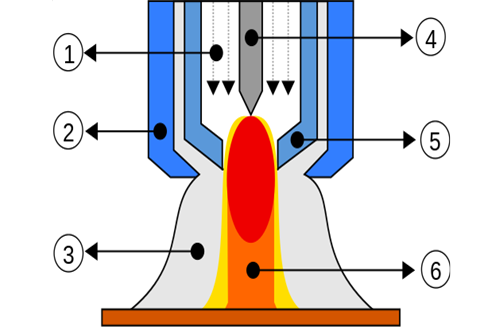
\includegraphics[width=\textwidth]{ptaTorc}
\end{figure}

\subsection{PTA’da kullanılan malzemeler}
PTA işlemi sırasında uygulanan akım, toz besleme hızı, ilerleme hızı ve plazma gaz debisi ortaya çıkan kaplamanın özelliklerini etkilemektedir. Kaplamalarda kullanılan toz malzemelerin ve yukarıda bahsedilen özelliklerin optimum dengede olması PTA kaplamasının istenen özellikleri sağlaması için önemlidir. PTA işlemi ile ilgili özellikler kullanılan kaplama tozuna karar verilmesinden sonra optimize edilmektedir. Kaplama için kullanılacak tozların da çeşitli kısıtları vardır [4]. 
1. Tozun tane boyutu 50µm ile 150µm arasında olmalıdır. Bu sınırların dışındaki tane boyutları besleme sorunlarına sebep olmaktadır. 
2. Toz taneleri küresel ya da keskin köşeli (angular shape) olmalıdır. Fiber tane şekilleri beslemede sorun çıkartmaktadır.
3. Kaplama malzemesi ve kaynak havuzu yakın yoğunlukta olmalıdır. Yüksek yoğunlukta parçacıklar kaynak havuzunda çökme gösterebilir.
				
\newpage

\printbibliography[ title={KAYNAKLAR\space DİZİNİ}] %numaralı olsun istersen optionlarda heading=bibnumbered, yaz
\defbibheading{bibliography}[\refname]{%
  \section*{#1}%
  \markboth{\MakeUppercase{#1}}{\MakeUppercase{#1}}}

\end{document}